% !TEX root = ../paper.tex
\section{System Architecture}
\label{sec:architecture}

The simulation state is partitioned into three cooperating subsystems, each
with distinct mutability semantics (Fig.~\ref{fig:architecture}).

\subsection{Snowpack (Static)}

The snowpack is a read-mostly Structure-of-Arrays (SoA) containing $10^6$
particles with positions, radii, masses, wetness values, and an \texttt{alive}
flag (\texttt{AVAILABLE}/\texttt{CONSUMED}). Positions are immutable after
initialisation; only the \texttt{alive} flag is toggled atomically upon
capture. The array is sorted once by \texttt{posX} to enable binary-search
range limiting.

\subsection{Shell (Dynamic)}

The shell is a fully dynamic SoA (\texttt{ParticleSystem}) storing positions,
velocities, forces, masses, radii, state flags, wetness, and body-frame
attachment vectors (\texttt{attachLocal}). Its capacity starts at 256 and
\textbf{grows dynamically} (doubling) as particles are captured, using
\texttt{cudaMalloc}/\texttt{cudaMemcpy} with the old buffer freed after copy.
Under steady-state conditions (1M snowpack, default parameters), the shell
stabilises at approximately 4{,}000 active particles.

\subsection{Core (Rigid Body)}

The snowball core is a single \texttt{SnowballState} struct maintained on the
host: position, velocity, quaternion orientation, angular velocity, mass, and
radius. It is updated each frame via rigid-body slope dynamics with rolling
and aerodynamic drag. Mass and radius grow as captured particles contribute
mass, with the radius derived as $R = (3m / 4\pi\rho)^{1/3}$.

\begin{figure}[H]
  \centering
  \fbox{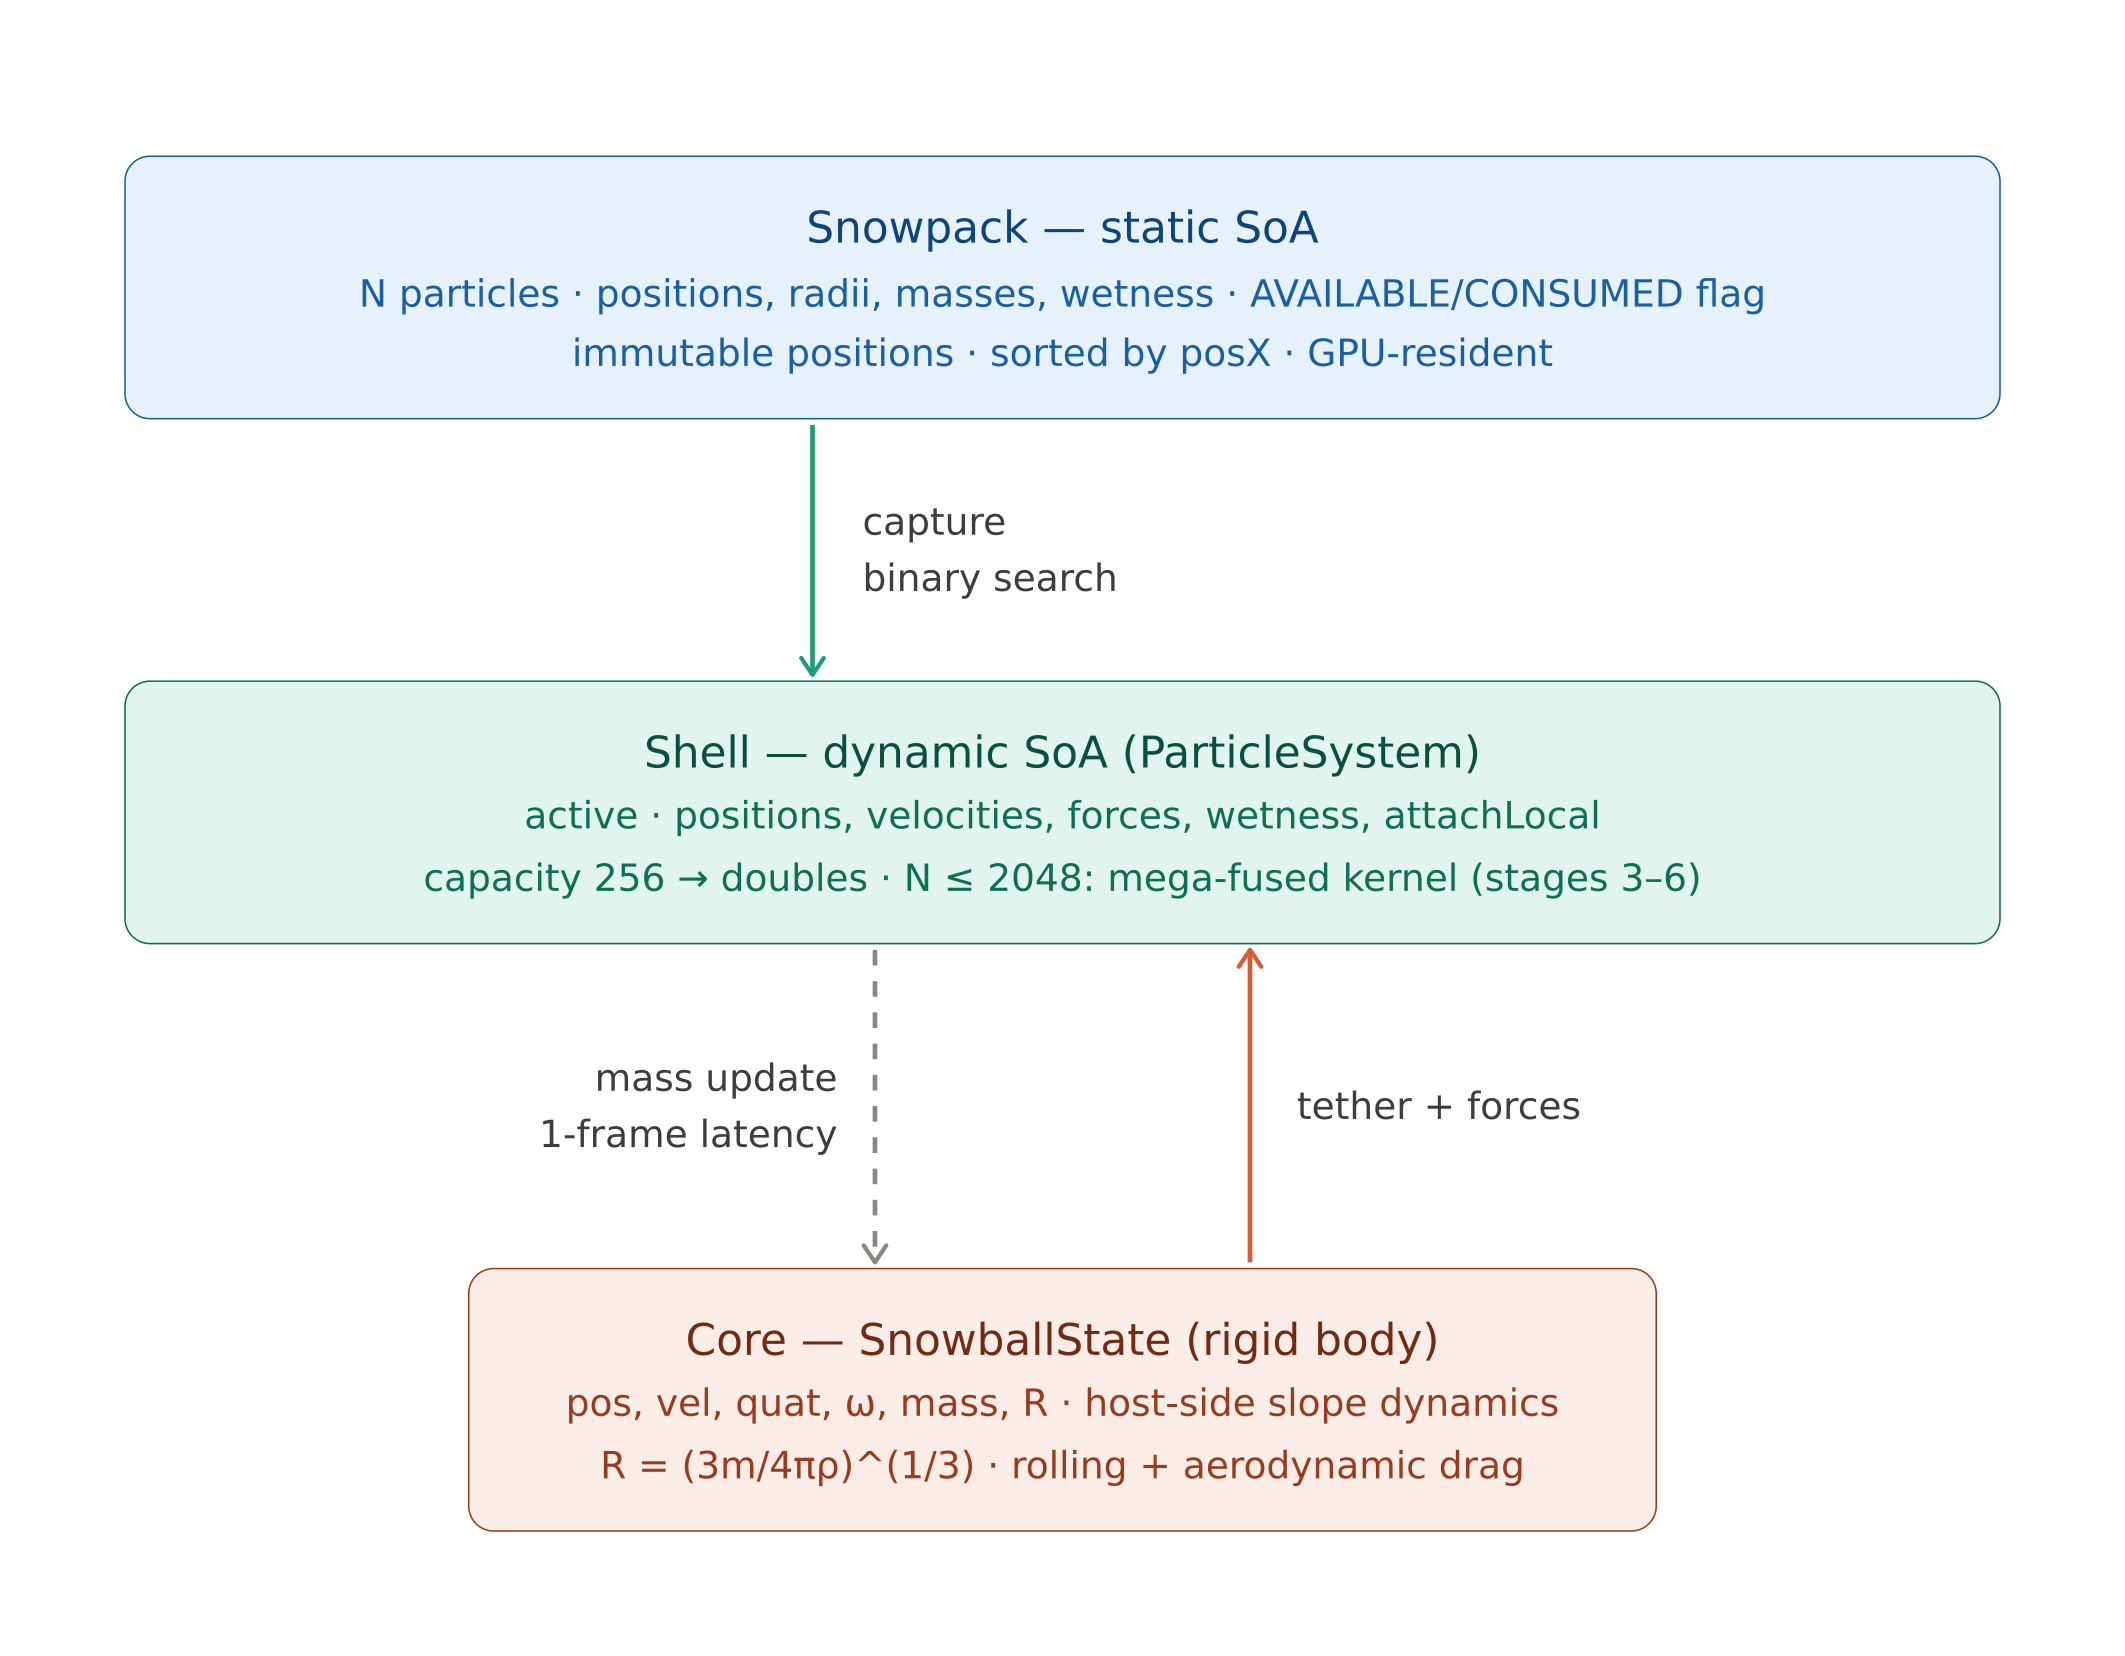
\includegraphics[width=0.9\columnwidth]{figures/architecture.png}}
  \caption{Three-tier particle architecture. The capture kernel converts
  snowpack particles into shell particles; each shell particle is tethered to
  the rigid-body core via a spring-damper.}
  \label{fig:architecture}
\end{figure}

\subsection{Per-Frame Data Flow}
\label{sec:dataflow}

The per-frame pipeline proceeds as follows:

\begin{enumerate}
  \item \textbf{Capture}: snowpack $\to$ shell (range-limited binary search).
  \item \textbf{Core mass update}: deferred readback (1-frame latency) of
        capture counters from device; momentum-conserving velocity scaling.
  \item \textbf{Forces + Tether}: gravity, damping, and tether spring
        (fused kernel).
  \item \textbf{Grid build}: spatial hash, CUB radix sort, cell ranges
        (\emph{parallel stream}).
  \item \textbf{Collision}: neighbour DEM + cohesion.
  \item \textbf{Integrate + Ground}: semi-implicit Euler + slope constraint
        (fused kernel).
  \item \textbf{Core rigid-body update}: host-side slope dynamics.
\end{enumerate}

For small shell counts ($N \leq 2048$), stages 3--6 are replaced by a
single \textbf{mega-fused kernel} that performs the entire physics pipeline
in one launch (Section~\ref{sec:mega_fused}).

\subsection{Deferred Capture Readback}
\label{sec:deferred}

Capture counters (particle count and accumulated mass) reside in a packed
8-byte device buffer, reset each frame via \texttt{cudaMemsetAsync}. The
result is read back asynchronously to pinned host memory. The host processes
the readback at the top of the \emph{next} frame (1-frame latency, physically
negligible at 300\,Hz). When more threads passed the probabilistic test than
the per-frame cap allows, the credited mass is scaled proportionally:
%
\begin{equation}
  m_{\text{credited}} = m_{\text{total}} \cdot
  \frac{\text{actualNew}}{\text{d\_captureCount}},
  \label{eq:mass_scaling}
\end{equation}
%
preventing the ball radius from inflating and triggering a runaway feedback
loop.
